%%---------------------------------------------------------------------
%	Preamble
%	AMS gruppe 12
%	AMS F18
%---------------------------------------------------------------------
\documentclass[12pt,fleqn,a4paper]{article}
\usepackage[utf8]{inputenc}
\usepackage[danish]{babel}
\usepackage[top=2.5cm, left=2cm, right=2cm, bottom=2.5cm]{geometry}
\usepackage{graphicx}
\usepackage[bottom]{footmisc}
\usepackage{framed}
\usepackage{caption}
\usepackage{float}
\usepackage{mdframed}
\usepackage{listings}
\usepackage{color}
\usepackage[T1]{fontenc}
\usepackage{amsmath,amsfonts,amsthm} % Math packages
\usepackage{array}
\usepackage{wrapfig}
\usepackage{multirow}
\usepackage{tabu}
\usepackage{longtable}
\usepackage{lastpage}
\usepackage{fancyhdr}
\usepackage[compact]{titlesec}
\usepackage[table,xcdraw]{xcolor}
\usepackage{arydshln}
\usepackage[isbn,issn,url]{dk-bib}
\usepackage[toc,page]{appendix}
\usepackage{url}
\def\UrlBreaks{\do\/\do-}

\definecolor{mygreen}{RGB}{28,172,0} % color values Red, Green, Blue
\definecolor{mylilas}{RGB}{170,55,241}
\renewcommand{\lstlistingname}{Kodeudsnit}
\tabulinesep=3mm

\setcounter{secnumdepth}{2}
\setcounter{tocdepth}{2}

\setlength{\parindent}{0mm} %intet indryk
\setlength{\parskip}{3mm} 	%linjeskift v. afsnit

% Ændring af enumerize og itemize 
\usepackage{enumitem} % @http://ctan.org/pkg/enumitem
\setlist[itemize]{topsep=0pt, itemsep=0.5pt}
\setlist[enumerate]{topsep=0pt, itemsep=0.5pt}

%afstand omkring sections
\titlespacing{\section}{0pt}{5mm}{0pt}
\titlespacing{\subsection}{0pt}{2mm}{0pt}
\titlespacing{\subsubsection}{0pt}{2mm}{0pt}

\usepackage{arydshln}
%aryd
\setlength\dashlinedash{3pt}
\setlength\dashlinegap{4pt}

\lstset{language=C++,
	breaklines=true,
	keywordstyle=\color{blue},
	stringstyle=\color{red},
	commentstyle=\color{mygreen},
	morecomment=[l][\color{magenta}]{\#}
}

%header & footer
\makeatletter
\pagestyle{fancy}
\fancypagestyle{plain}{}
\renewcommand{\chaptermark}[1]{\markboth{#1}{}}
\setlength{\headheight}{35pt}
\fancyfoot{} % clear all fields
\fancyfoot[R]{Side \thepage\ af \pageref{LastPage}}
\fancyhead{} % clear all fields
\fancyhead[L]{
\includegraphics[clip, trim = 0 0 240pt 0, height=30pt]{Figur/IHA_AU_logo.png}}
\fancyhead[R]{Forår 2018}
\fancyhead[C]{Anvendte Microcontroller Systemer}
\renewcommand{\headrulewidth}{0pt}

\def\thickhrulefill{\leavevmode \leaders \hrule height 1.2ex \hfill \kern \z@}
\def\@makechapterhead#1{
  \vspace*{10\p@}%
  {\parindent \z@ \centering \reset@font
        \thickhrulefill\quad 
        \scshape\bfseries\textit{\@chapapp{}  \thechapter}  
        \quad \thickhrulefill
        \par\nobreak
        \vspace*{10\p@}%
        \interlinepenalty\@M
        \hrule
        \vspace*{10\p@}%
        \Huge \bfseries #1 \par\nobreak
        \par
        \vspace*{10\p@}%
        \hrule
        \vskip 40\p@
  }}

\usepackage{tcolorbox}
\definecolor{mycolor}{rgb}{0.122, 0.435, 0.698}% Rule colour
\makeatletter
\newcommand{\mybox}[1]{%
	\setbox0=\hbox{#1}%
	\setlength{\@tempdima}{\dimexpr\wd0+13pt}%
	\begin{tcolorbox}[colframe=mycolor,boxrule=0.5pt,arc=4pt,
		left=6pt,right=6pt,top=6pt,bottom=6pt,boxsep=0pt]
		#1
	\end{tcolorbox}
}
\makeatother

\graphicspath{ {Figur/} }


%Se Kodeudsnit \ref{lstlisting:generel_kode}

%\captionof{lstlisting}{Generelle egenskaber for koden til fremstilling af diverse figure i matlab} 
%\label{lstlisting:generel_kode}
%\vspace{5mm} %5mm vertical space
%
%\subsection{Kode til lyd i forhold til tiden}
%\begin{framed}
%\begin{center}
%\begin{lstlisting}
%figure('name','trafikstoejen i fuld laengde'); clf
%subplot(211);
%plot(t,s_sound_left)
%xlabel('Tid (sek)')
%ylabel('Signalstyrke')
%title('Trafikstoej set i forhold til tiden')
%grid on
%hold on
%\end{lstlisting}
%\end{center}
%\end{framed}




%\begin{document}

\section{Skærm}
Skærmen er den grafiske brugergrænseflade til systemet. Den skal give brugeren en grafisk præsentation af lydinputtet i mikrofonen. Lyden bliver vist på skærmen ved hjælp af et spektrogram der er 40 pixels bredt, og 240 pixels højt.
Skærmen er inddelt i 8 søjler på hver 40 pixels. Den første søjle viser farvespektret hvor det kan ses hvilken farve der beskriver lyddensiteten. De sidste syv søjler viser spektret over det aktuelle lydbillede. Se figur \ref{fig:skaerm_spectrum}

\begin{figure} [H]
	\centering
	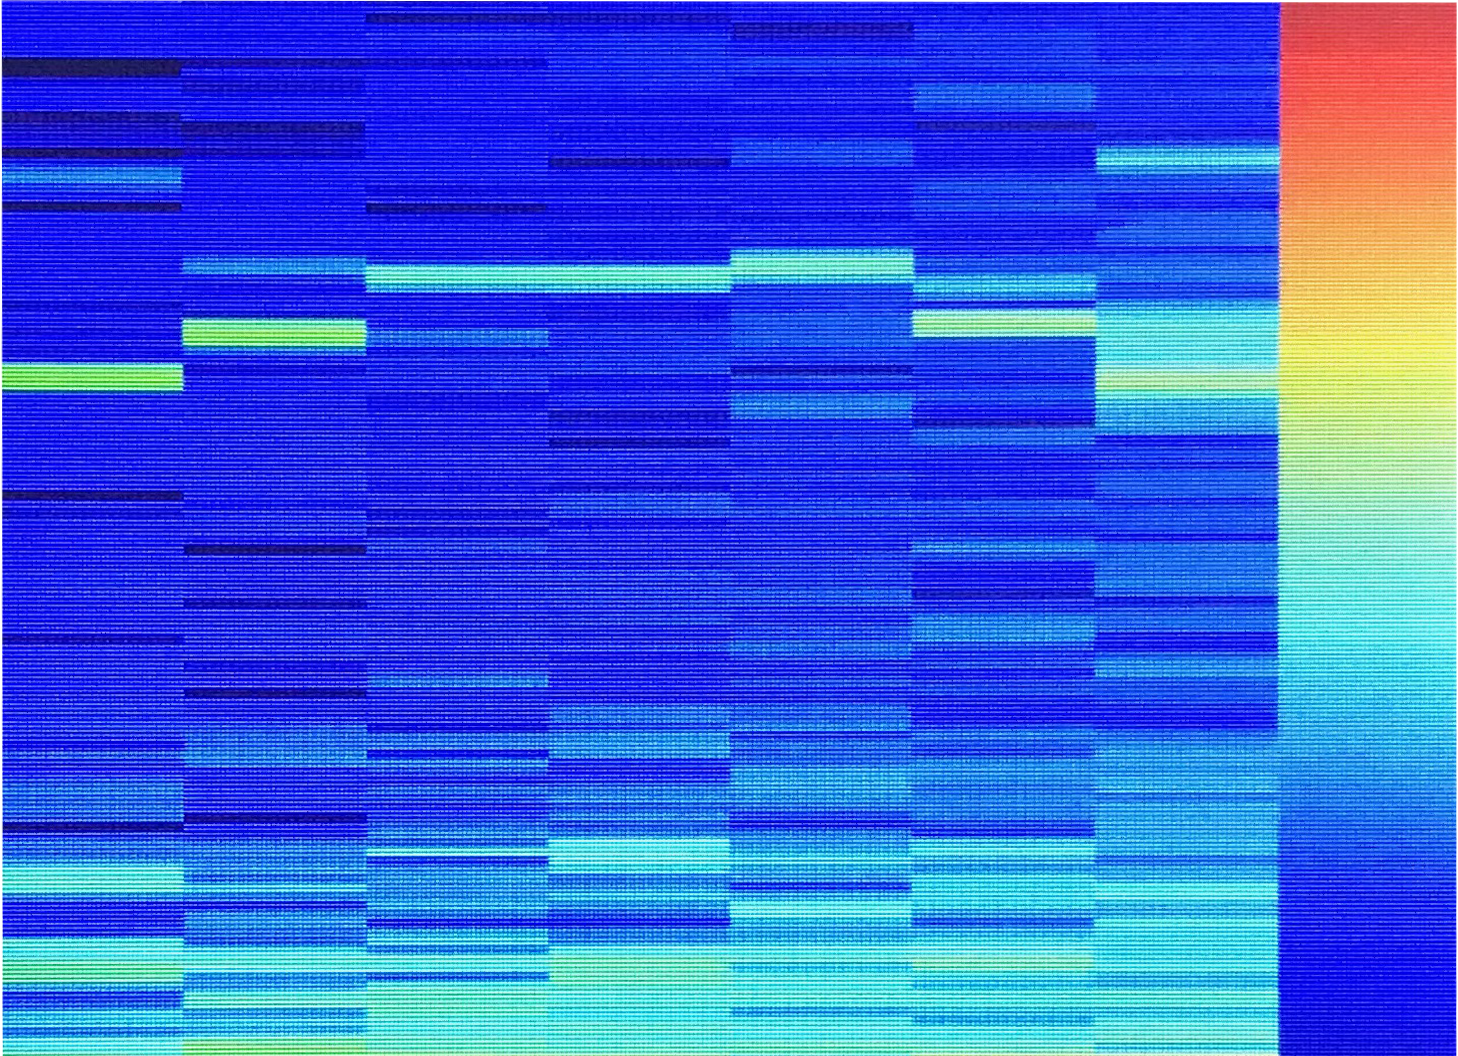
\includegraphics[width=0.7 \textwidth]{skaerm_spectrum.png}
	\captionof{figure}{Brugergrænsefladen med 8 søjler. 7 der hver repræsenterer lydbilledet for tiden, og en der viser farvespektret}
	\label{fig:skaerm_spectrum}
\end{figure}

\subsection{Farve}
Farverne som den aktuelle spektrogram søjle der vises, bliver valgt ud fra outputtet fra FHT modulet. Outputtet fra FHT modulet er et array med 128 pladser der hver indeholder et tal mellem 0 og 255. 0 betyder lav densitet og 255 betyder høj.
For at få dette tal repræsenteret som en farve på displayet, skal tallet omsættes til en RGB565 kode.
Dette er gjort ved at lave en lookup table på 3X256 pladser, som et python script autogenerer og derved laver en c fil.

\begin{figure} [H]
	\centering
	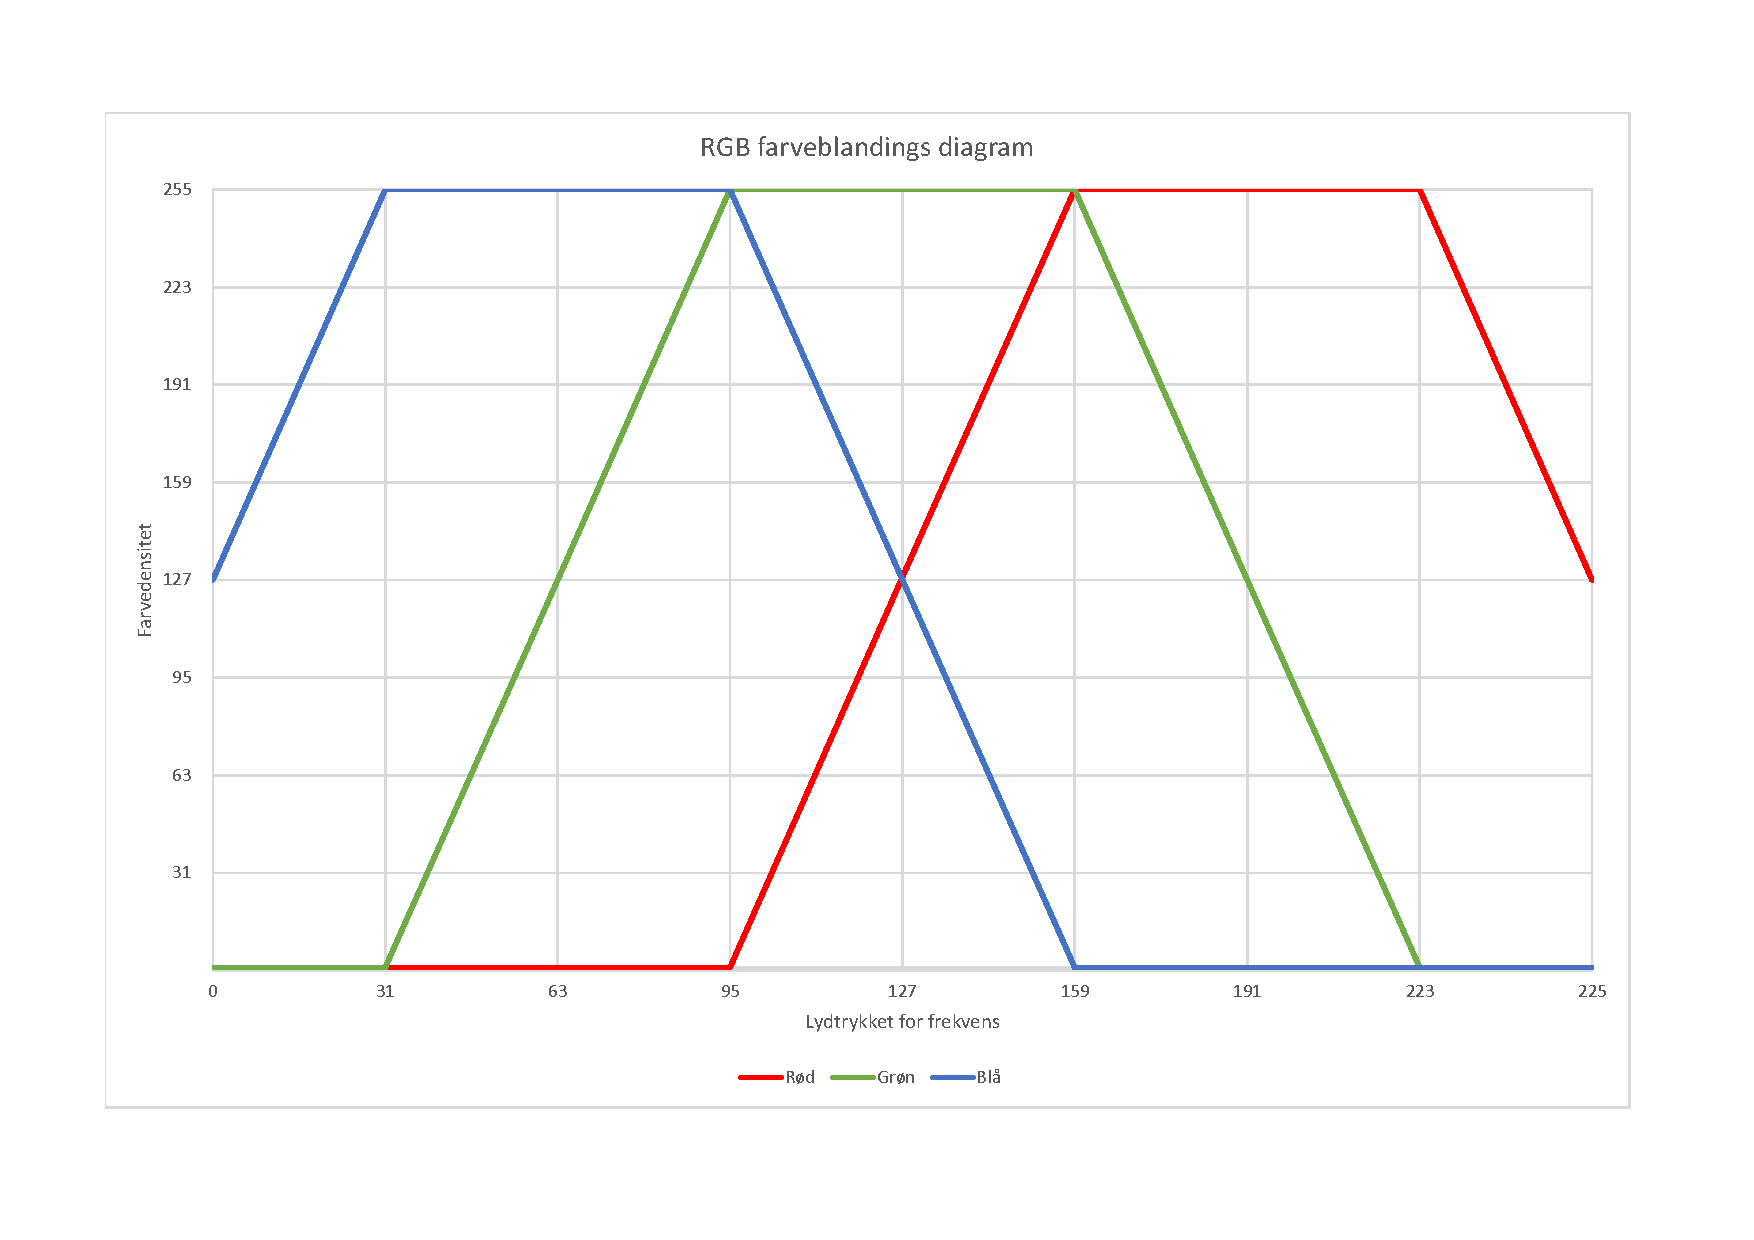
\includegraphics[width=0.7 \textwidth, trim={0cm, 2cm, 0cm, 1.8cm}, clip]{rgb_diagram.pdf}
	\captionof{figure}{RGB farveblandingsdiagram der bliver brugt til algoritmen til lookup table}
	\label{fig:rgb_diagram}
\end{figure}


På figur \ref{fig:rgb_diagram} ses diagrammet over farveblandingen der bliver brugt til at lave lookup tabellen. X-aksen er det tal der bliver slået op med, altså outputtet fra FHT modulet. Y-aksen viser RGB koden.


\subsection{Skærmdriver}
Det viste billede på skærmen skal hele tiden flytte søjlerne én plads til venstre (x-aksen), og skrive en ny søjle ud til højre. Søjlen helt til højre skal vise farvespektret konstant.
Y-aksen repræsenterer frekvenserne fra 500 Hz op til 10 kHz. se figur \ref{fig:skaerm_spectrum_forklaring}.

\begin{figure} [H]
	\centering
	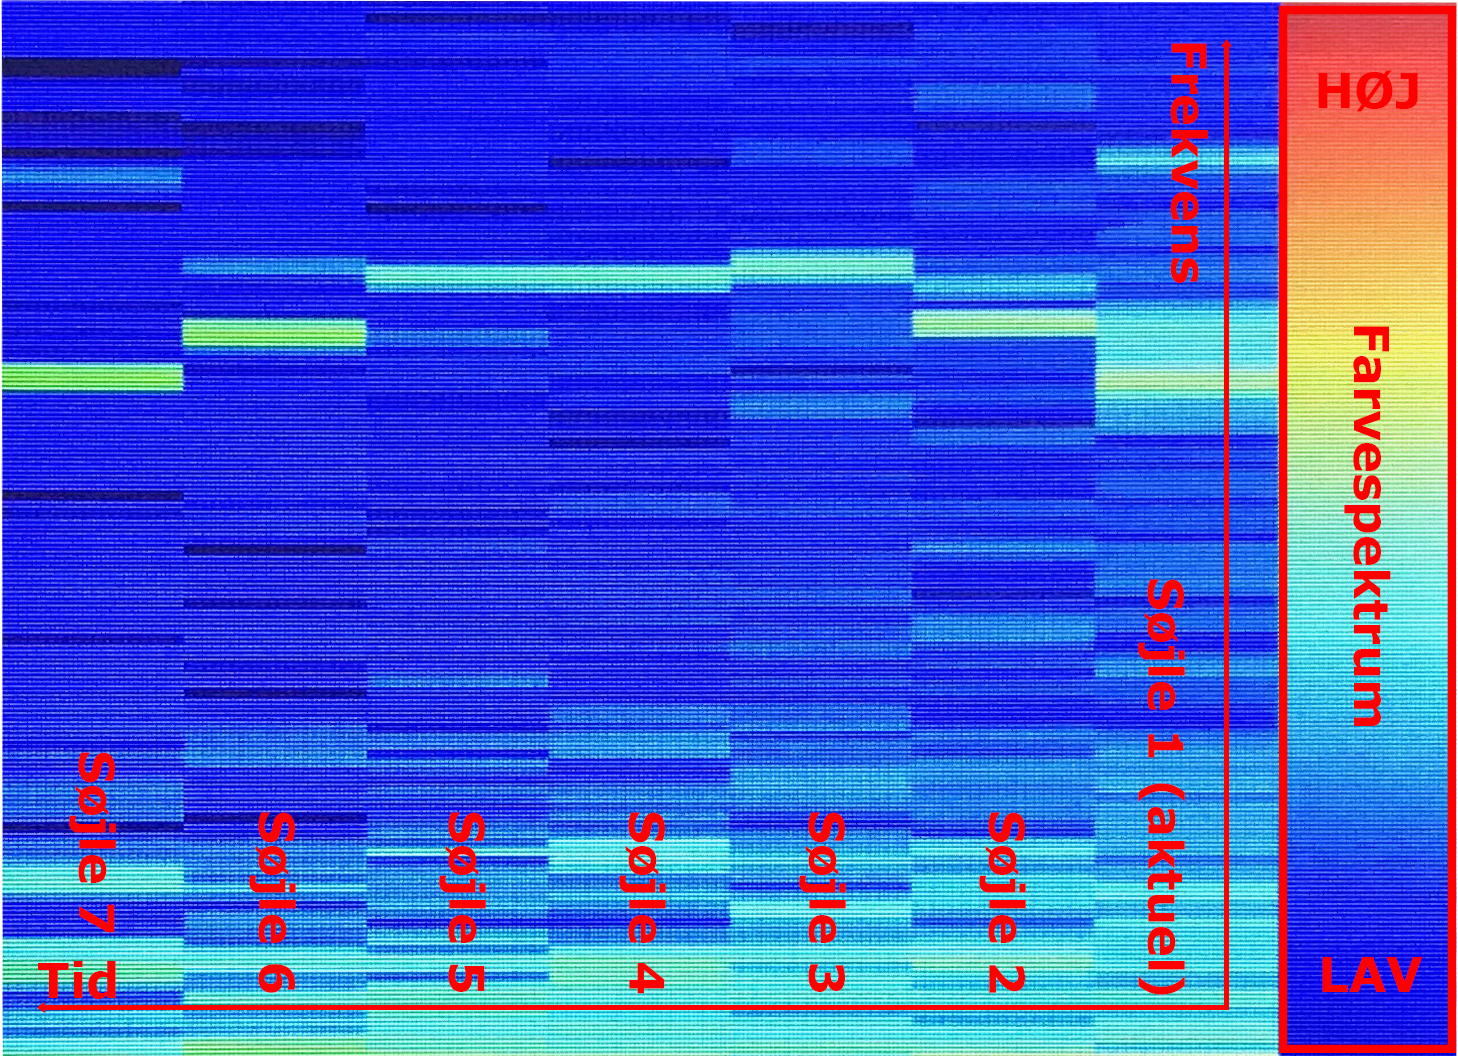
\includegraphics[width=0.7 \textwidth]{skaerm_spectrum_forklaring.png}
	\captionof{figure}{Søjlerne flytter hele tiden én plads til venstre, så en ny søjle kan tegnes på skærmen. Y-aksen viser en farve der repræsenterer lydstyrken for hver frekvens}
	\label{fig:skaerm_spectrum_forklaring}
\end{figure}

Skærm driveren har taget udgangspunkt i den driver der blev lavet i lab3, men er blevet modificeret til dette projekts behov. 
Der er derfor lavet fire nye funktioner i driveren:
\begin{itemize}
	\item \textit{DrawLine} Skal tegne en linje der er én pixel høj.
	\item \textit{InitScrolling} Skal initiere scrolling på skærmen.
	\item \textit{MoveDisplay} Skal flytte den gamle søjle én plas, så der kan skrives en ny på skærmen.
	\item \textit{UpdateDisplayPointer} skal fortælle skærmen hvor meget den skal flyttes.
\end{itemize}

\subsubsection{DrawLine}
To linjer repræsenterer én frekvens. Derfor skulle der bruges en funktion der kunne tegne én linje på en given bredde med en farve der repræsenter lyd intensiteten.
Funktionen er derfor lavet således at den får et X, Y koordinat med hvor den skal starte med at tegne, længden på linjen, der i dette projekts tilfælde altid er 40 pixels, og til sidst RGB565 farvekoden.

\subsubsection{InitScrolling}
Skærmen skal hele tiden opdatere sig selv, ved at rykke søjlerne én plads til venstre, og tegne en ny i højre side. For at undgå at skrive hele skærmen om for hver opdatering, bliver funktionen "Vertical Scrolling" fra ILI9341 udnyttet.

Figur \ref{fig:scrolling} viser grafisk hvordan skærmen inddeles når scrolling effekten bruges. Eftersom denne skærm skal have en konstant søjle i højre side (set som bunden i forhold til ILI9341) med farvespektret, er der derfor valgt at have "fixed area", i dette tilfælde BFA.

\begin{figure} [H]
	\centering
	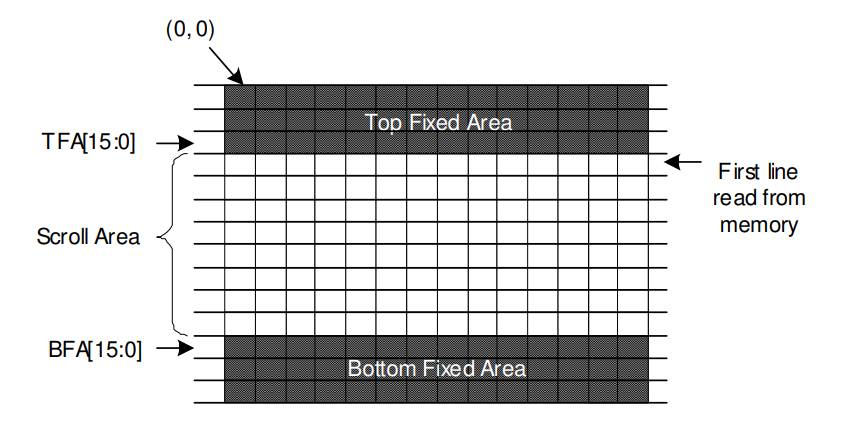
\includegraphics[width=0.7 \textwidth]{scrolling.png}
	\captionof{figure}{Grafisk billede på hvordan skærmen er opdelt når scrolling effekten bruges}
	\label{fig:scrolling}
\end{figure}

Figur \ref{fig:scrolling_kommandoer} viser hvordan vertical scrolling initieres, og hvilke parametre der sendes.
Der skal altså skrives en kommando (0x33) først, og derefter seks parametre. I dette tilfælde er de seks parametre:
De første to er 0, da der ikke skal være et fixed area i venstre side (toppen). De næste to er 280 (0x01 og 0x18), da skærmen er 320 pixels bred, og 40 af dem skal reserveres til farvespektret i højre side. De sidste to parametre er 40 (0x00 og 0x28), hvilket er det fixed area der skal være i højre side (bunden).

\begin{figure} [H]
	\centering
	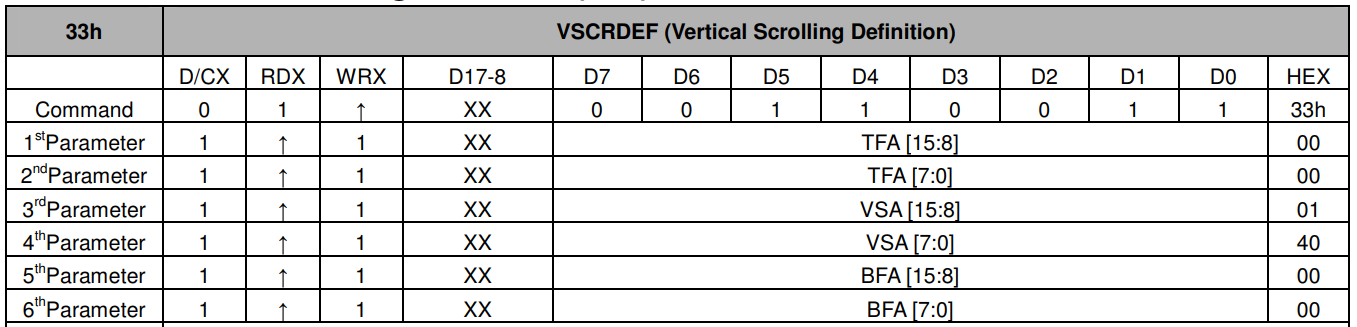
\includegraphics[width=0.7 \textwidth]{scrolling_kommandoer.png}
	\captionof{figure}{Tabellen der viser hvordan vertical scrolling initieres}
	\label{fig:scrolling_kommandoer}
\end{figure}

\subsubsection{MoveDisplay}
Funktionen MoveDisplay er den funktion der får skærmbilledet til at scrolle. Denne funktion opdaterer scrolling startadressen. Funktionen skal altså kaldes hver gang skærmbilledet skal flyttes en plads til venstre. 

\subsubsection{UpdateDisplayPointer}
For at få skærmbilledet til at flytte 40 pixels hver gang der skal udskrives nyt data, er der brug for en funktion der kan hæve startadressen med 40 pixels hver gang, Ellers ville skærmens startadresse være den samme, og skærmen ville derfor ikke flytte sig. Dette gøres ved at hæve det tal der bruges i MoveDisplay til at flytte startadressen med de antal pixels skærmen ønskes at flyttes. Der bliver i denne funktion også taget højde for at der ikke kan scrolles længere ud end skærmen er bred. Variablen skal derfor resettes hvis den bliver højere en de 320 pixels som skærmen er bred.

\subsection{Billeddriver}
Der er lavet en driver til at tegne billedet på skærmen. Denne driver indeholder to funktioner:
\begin{itemize}
	\item \textit{DisplayGradient} Skal tegne farvespektret i højre side.
	\item \textit{DrawBins} Skal tegne to linjer der repræsenterer ét frekvensbin.
\end{itemize}

\subsubsection{DisplayGradient}
Denne funktion skal tegne søjlen med farvespektret i højre side. Det gør den ved at tegne en linje ad gangen, startende fra 0 og op, med den RGB565 kode der hører til det linjenummer den tegner.
Dette vil give en pæn gradient hvor farven der repræsenterer 0 (dyb blå) er nederst, og den farve der repræsenterer den højeste densitet (Rød) er øverst.

\subsubsection{DrawBins}
Denne funktion tegner to linjer der repræsenterer et frekvensbin med den farve der beskriver lydstyrken. Outputtet fra FHT modulet giver de tal der beskriver lydstyrken for hver bin, og de kan derfor oversættes ved hjælp af lookup tabellen, der blev autogenereret af et python script, til den RGB565 kode der skal vises på skærmen.

\subsection{Test}
For at teste driverne til skærmen er der lavet et "dummy array" der skal simulere outputtet fra FHT modulet. Dette array lavet ved at lade et python script autogenere en c fil "DummyFHT.c". Denne fil indeholder er array (fht\_log\_out) med 128 pladser, med hver et random tal mellem 0 og 255. Disse tal repræsenterer en farve der skal vises på skærmen ved hjælp af lookup tabellen med RGB565 koderne.


%\end{document}